% !TEX program = xelatex
% !TEX encoding = UTF-8
% !BIB program = bibtex
% !TEX spellcheck = en_US
\documentclass[12pt]{article}
\usepackage[letterpaper, margin=1in]{geometry}
\usepackage{amsmath,amssymb}
\usepackage{graphicx}
\usepackage{subfigure}
\usepackage{newpxtext,newpxmath}
\usepackage{siunitx}
\usepackage{hyperref}
\usepackage{bm}
\usepackage[version=4]{mhchem}
\usepackage{tikz}
\usetikzlibrary{calc}
\usetikzlibrary{arrows.meta}
\usetikzlibrary{decorations.pathreplacing}
\usetikzlibrary{decorations.pathmorphing}
\usepackage{relsize}
\tikzset{fontscale/.style = {font=\relscale{#1}}
}
\usepackage{wrapfig}
\usepackage{lipsum}

\makeatletter
\newcommand{\gettikzxy}[3]{%
  \tikz@scan@one@point\pgfutil@firstofone#1\relax
  \edef#2{\the\pgf@x}%
  \edef#3{\the\pgf@y}%
}
\makeatother

\newcommand{\tikzmark}[1]{\tikz[overlay,remember picture] \node (#1) {};}

\begin{document}
\setcounter{section}{12}
\section{Spinodal Decomposition}

Consider a binary alloy system with a miscibility gap,
i.e.,
\begin{figure}[h]
	\begin{minipage}[l]{0.3\textwidth}
		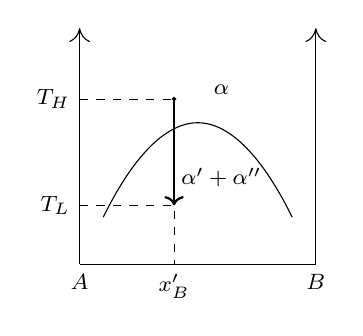
\begin{tikzpicture}[scale=3, font=\footnotesize]
	% axis
	\draw [-{>[scale=2.5,
    length=2,
    width=3]}] (0,0) -- (0,1);
	\draw (0,0) -- (1,0);
	\draw [-{>[scale=2.5,
    length=2,
    width=3]}] (1,0) -- (1,1);

	% curve
	\coordinate (A) at (0.1,0.2);
	\coordinate (B) at (0.9,0.2);
	\draw (A) parabola[bend pos=0.5] bend +(0,0.4) (B);

	% line
	\coordinate (xb') at (0.4,0);
	\coordinate (TL) at (0,0.25);
	\coordinate (TH) at (0, 0.7);
	\draw[dashed] (TL) -| (xb');
	\draw[dashed] (TH) -- ($ (xb') + (TH) $);

	% arrow
	\draw[->, thick] ($ (xb') + (TH) $) -- ($ (xb') + (TL) $);

	% point
	\draw[fill=black] ($ (xb') + (TH) $) circle[radius=0.2pt];

	% text
	\draw (TH) node[anchor=east] {$T_H$};
	\draw (TL) node[anchor=east] {$T_L$};
	\draw (0.6,0.45) node[anchor=north] {$\alpha'+\alpha''$};
	\draw (0.6,0.8) node[anchor=north] {$\alpha$};
	\draw (xb') node[anchor=north] {$x_B'$};
	\draw (0,0) node[anchor=north] {$A$};
	\draw (1,0) node[anchor=north] {$B$};
\end{tikzpicture}
	\end{minipage}%
	\hfil
	\begin{minipage}[r]{0.6\textwidth}
		now, consider a transformation which must occur when an alloy
		with composition $x_B'$ is quenched from temperature $T_H$
		to a lower temperature $T_L$', i.e.,
		\begin{equation*}
			\ce{$\alpha$ -> $\alpha' + \alpha''$}.
		\end{equation*}
	\end{minipage}
\end{figure}

In order to properly deal with the transformation, we need to analyze,
not surprisingly, the $G_{\text{sol}}$ vs composition relation at the
transformation temperature $T_L$!

I.e.,
\begin{figure}[h]
	\begin{minipage}[l]{0.3\textwidth}
		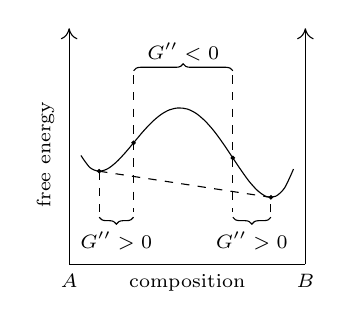
\begin{tikzpicture}[scale=3, domain=0.05:0.95, font=\scriptsize]
	% axis
	\draw [-{>[scale=2,
			length=2,
			width=3]}] (0,0) -- (0,1);
	\draw (0,0) -- (1,0);
	\draw [-{>[scale=2,
			length=2,
			width=3]}] (1,0) -- (1,1);

	\begin{scope}[yscale=0.5, yshift=0.5cm]
		% curve
		\coordinate (g00A) at (0.272815, 0.529808);
		\coordinate (g00B) at (0.692895, 0.402102);
		\coordinate (g0A) at (0.127138, 0.289339);
		\coordinate (g0B) at (0.854233, 0.0681958);
		\draw plot[smooth] (\x, {0.7 - 7.45598 * \x + 41.666 * \x^2 - 70.9531 * \x^3 + 36.7362 * \x^4});
	\end{scope}


	% line
	\gettikzxy{(g00A)}{\ax}{\ay};
	\gettikzxy{(g00B)}{\bx}{\by};
	\gettikzxy{(g0A)}{\fax}{\fay};
	\gettikzxy{(g0B)}{\fbx}{\fby};
	\draw[dashed] (\ax, 0.8) -- (\ax, 0.22);
	\draw[dashed] (\bx, 0.8) -- (\bx, 0.22);
	\draw[dashed] (g0A) -- (g0B);
	\draw[dashed] (\fax, \fay) -- (\fax, 0.22);
	\draw[dashed] (\fbx, 0.22) -- (\fbx, \fby);

	% point
	\draw[fill=black] (g00A) circle[radius=0.2pt];
	\draw[fill=black] (g00B) circle[radius=0.2pt];
	\draw[fill=black] (g0A) circle[radius=0.2pt];
	\draw[fill=black] (g0B) circle[radius=0.2pt];

	% text
	\draw (0.5, 0) node[anchor=north] {composition};
	\draw (0,0) node[anchor=north] {$A$};
	\draw (1,0) node[anchor=north] {$B$};
	\draw (-0.1,0.2) node[anchor=west, rotate=90] {free energy};
	\draw ($ ( {(\ax + \bx)/2}, 0.9) $) node (g) {$G'' < 0$};  % You need to wrap the expression into { } to hide the second pair of ( ) from the TeX parser.
	\draw ($ ( {(\fax + \ax)/2}, 0.1) $) node (g) {$G'' > 0$};
	\draw ($ ( {(\fbx + \bx)/2}, 0.1) $) node (g) {$G'' > 0$};

	% others
	\draw [
		decoration={
				brace
			},
		decorate
	] (\ax,0.82) -- (\bx,0.82);
	\draw [
		decoration={
				brace,
				mirror,
			},
		decorate
	] (\fax, 0.2) -- (\ax, 0.2);
	\draw [
		decoration={
				brace,
			},
		decorate
	] (\fbx, 0.2) -- (\bx, 0.2);
\end{tikzpicture}
	\end{minipage}%
	\hfil
	\begin{minipage}[r]{0.6\textwidth}
		In particular,
		\begin{enumerate}
			\item If $x_B'$ inside the $G''<0$ region, then small fluctuations
			      in composition $\Rightarrow G \downarrow$ about $x_B'$.
			      $\therefore$ system is unstable and decomposition continues via
			      ``uphill'' diffusion!
		\end{enumerate}
	\end{minipage}
\end{figure}

On the other hand,
\begin{enumerate}
	\setcounter{enumi}{1}
	\item If $x_B'$ outside the $G''<0$ region,
	      small variations in composition $\Rightarrow$ increase in the total
	      free energy of the system (i.e., $G \uparrow$).
	      $\therefore$ system is metastable and requires large fluctuations to
	      develop \ce{$\alpha' + \alpha''$} (i.e., N and G required here).
\end{enumerate}

Expand $G(c)$ about $c_0$, then
\begin{align*}
	G(c_0 + \Delta c) & =
	G(c_0) + G'(c_0) \cdot \Delta c +
	G''(c_0) \cdot \frac{ (\Delta c)^2 }{ 2! }
	+ \cdots,\\
	G(c_0 - \Delta c) & =
	G(c_0) - G'(c_0) \cdot \Delta c +
	G''(c_0) \cdot \frac{ (\Delta c)^2 }{ 2! }
	+ \cdots.
\end{align*}
\begin{equation*}
	\therefore \Delta G = \frac{ G(c_0 + \Delta c) + G(c_0 - \Delta c) }{ 2 }
	- G(c_0) = \frac{ G''(c_0) (\Delta c)^2 }{ 2 },
\end{equation*}
which is to say that $\Delta G < 0$ if $G''(c_0) < 0$ and $\Delta G > 0$ if
$G''(c_0) > 0$.

If we plot $G'' = 0$ points at various temperature, we obtain the chemical
spinodal (i.e., line of $G'' = 0$).

\begin{figure}[h]
	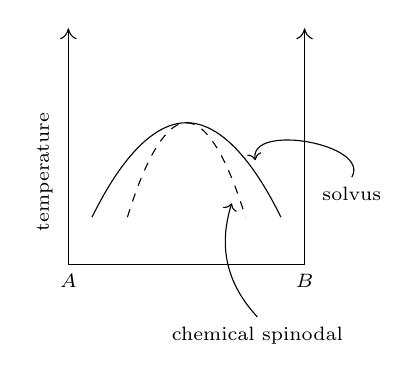
\begin{tikzpicture}[scale=3, font=\scriptsize]
	% axis
	\draw [-{>[scale=2,
			length=2,
			width=3]}] (0,0) -- (0,1);
	\draw (0,0) -- (1,0);
	\draw [-{>[scale=2,
			length=2,
			width=3]}] (1,0) -- (1,1);

	% curve
	\coordinate (A) at (0.1,0.2);
	\coordinate (B) at (0.9,0.2);
	\coordinate (C) at (0.25,0.2);
	\coordinate (D) at (0.75,0.2);
	\draw (A) parabola[bend pos=0.5] bend +(0,0.4) (B);
	\draw[dashed] (C) parabola[bend pos=0.5] bend +(0,0.4) (D);

	% node
	\draw (0,0) node[anchor=north] {$A$};
	\draw (1,0) node[anchor=north] {$B$};
	\draw (-0.1,0.1) node[anchor=west, rotate=90] {temperature};
	\draw (0.8, -0.3) node (n1) {chemical spinodal};
	\draw (1.2, 0.3) node (n2) {solvus};
	\draw (0.65, 0.3) node (ns1) {}; % chemical spinodal
	\draw (0.75, 0.4) node (ns2) {}; % solvus

	% reference
	\path[->] (n1.north) edge [out=180, in=0, bend left] (ns1.south east);
	\path[->] (n2.north) edge [out=60, in=100] (ns2.north east);
\end{tikzpicture}
\end{figure}

\newpage
Inside the spinodal $\rightarrow$ spontaneous decomposition can occur
via ``uphill'' diffusion process, i.e.,
\begin{figure}[h]
	\centering
	\begin{minipage}[b]{.5\linewidth}
		\centering
		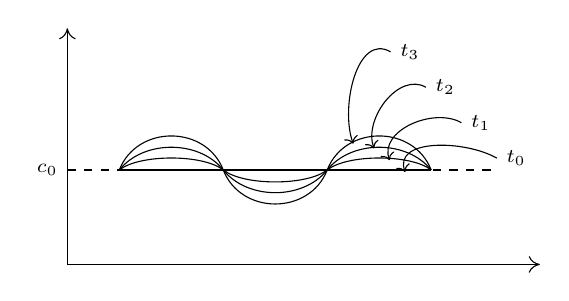
\begin{tikzpicture}[scale=3, font=\scriptsize]
	% axis
	\draw [-{>[scale=2,
			length=2,
			width=3]}] (0,0) -- (0,1);
	\draw[-{>[scale=2,
			length=2,
			width=3]}] (0,0) -- (2,0);

	% curve
	\begin{scope}[xscale=2.2, yshift=-0.1cm]
		\foreach \theta / \l in {0/0, 60/1, 70/1.75, 80/2.5}
		\draw (0.1,0.5) to [out=\theta, in=180-\theta, looseness=\l] (0.3,0.5)
		to [out=-\theta, in=\theta-180, looseness=\l] (0.5,0.5)
		to [out=\theta, in=180-\theta, looseness=\l] (0.7,0.5);
	\end{scope}

	\begin{scope}[yshift=-0.1cm]
  % line
  \draw[dashed] (0,0.5) -- (1.8,0.5);
  
  % node
  \draw (0,0.5) node[anchor=east] {$c_0$};
  \draw (2.2*0.65,0.45) node (c0) {};
  \draw (2.2*0.62,0.5) node (c1) {};
  \draw (2.2*0.59,0.55) node (c2) {};
  \draw (2.2*0.55,0.57) node (c3) {};
  \draw (1.9,0.55) node (t0) {$t_0$};
  \draw (1.75,0.7) node (t1) {$t_1$};
  \draw (1.6,0.85) node (t2) {$t_2$};
  \draw (1.45,1.0) node (t3) {$t_3$};
  
  % reference
  \path[->] (t0.west) edge [out=150, in=110] (c0.north);
  \path[->] (t1.west) edge [out=150, in=110] (c1.north);
  \path[->] (t2.west) edge [out=150, in=110] (c2.north);
  \path[->] (t3.west) edge [out=150, in=110] (c3.north);
  \end{scope}
\end{tikzpicture}
	\end{minipage}%
	\hfill
	\begin{minipage}[b]{.5\linewidth}
		\centering
		\begin{tikzpicture}[scale=3, font=\scriptsize, remember picture]
	% axis
	\draw [-{>[scale=2,
			length=2,
			width=3]}] (0,0) -- (0,1);
	\draw[-{>[scale=2,
			length=2,
			width=3]}] (0,0) -- (2,0);

	% line
	\begin{scope}[xscale=2.2, yshift=0.05cm]
		\draw (0.1,0.2) |- (0.3,0.5) |- (0.5,0.2) |- (0.7,0.5) -- (0.7,0.2);
		\draw[dashed] (0,0.2) -- (0.8,0.2);
		\draw[dashed] (0,0.5) -- (0.8,0.5);
		\draw[dotted] (0.71,0.55) -- (0.8,0.55);

		% node
		\draw (0,0.2) node[anchor=east] {$\alpha'$};
		\draw (0,0.5) node[anchor=east] {$\alpha''$};
		\draw (0.2,0.55) node[anchor=south] {$\alpha''$};
		\draw (0.4,0.55) node[anchor=south] {$\alpha'$};
		\draw (0.6,0.55) node[anchor=south] {$\alpha''$};
		\draw (0.75, 0.55) node[anchor=south] {etc.};

		% others
		\def\h{0.55}
		\def\marg{0.01}
		\draw [
			decoration={
					brace
				},
			decorate
		] (0.1+\marg,\h) -- (0.3-\marg,\h);
		\draw [
			decoration={
					brace,
				},
			decorate
		] (0.3+\marg,\h) -- (0.5-\marg,\h);
		\draw [
			decoration={
					brace,
				},
			decorate
		] (0.5+\marg,\h) -- (0.7-\marg,\h);
	\end{scope}
  
  % reference
  \draw (-0.2,0.5) node (f2) {}; % for reference
\end{tikzpicture}
	\end{minipage}
\end{figure}
\begin{tikzpicture}[remember picture, overlay, font=\scriptsize]
	\draw [->,decorate,decoration=snake] (f1) -- (f2);
	\gettikzxy{(f1)}{\faax}{\faay};
	\gettikzxy{(f2)}{\fbbx}{\fbby};
	\draw ($ ({(\faax+\fbbx)/2}, \faay) $) node[anchor=north] {eventually};
\end{tikzpicture}

\tikz[remember picture, inner sep=0pt] \node (f4) {};
Initially, no sharp and well defined boundaries. Instead, we have interfacial
regions which evolve and become sharper as the transformation proceeds.

\begin{tikzpicture}[remember picture,overlay]
	\draw[->] (f3) edge [out=180, in=160] (f4);
\end{tikzpicture}

Before review of thermodynamics/up-hill diffusion.
Recall $\bm{v} = M \bm{F} = - M \nabla \mu$, $\bm{J} = c \bm{v} = - M c \nabla \mu$, where
$M$ is mobility, $c$ is concentration, $\mu$ is chemical potential.
In 1D,
\begin{equation*}
	J = - M c \frac{ \partial \mu }{ \partial x } = - M c \frac{ \partial \mu }{ \partial c } \frac{ \partial c }{ \partial x } = - D \frac{ \partial c }{ \partial x },
\end{equation*}
\begin{equation*}
	\therefore D = M c \frac{ \partial \mu }{ \partial x },
\end{equation*}
where for $A-B$ binary system, $\mu_B = G_{\text{sol}} + (1-x_B)
	\Big( \frac{ dG_{\text{sol}} }{ dx_B } \Big)_{x_B'}$.
\begin{equation*}
	\frac{ d\mu_B }{ dx_B } = \frac{ dG_{\text{sol}} }{ dx_B } + (1-x_B)
	\frac{ d^2G_{\text{sol}} }{ dx_B^2 } +
	\Big( - \frac{ dG_{\text{sol}} }{ dx_B } \Big) =
	(1-x_B)
	\frac{ d^2G_{\text{sol}} }{ dx_B^2 },
\end{equation*}
\begin{equation*}
	\frac{ d\mu_i }{ dx_i } = (1-x_i) G''
\end{equation*}
and
\begin{equation*}
	\frac{ d\mu_i }{ dc_i } = (1-x_i) V_m \frac{ d^2G_{\text{sol}} }{ dx_i^2 }
\end{equation*}
since $c_i = \frac{ x_i }{ V_m } \Rightarrow V_m dc_i = dx_i$.
And finally
\begin{equation*}
	D_i = M_i c_i V_m (1-x_i) \frac{ d^2G_{\text{sol}} }{ dx_i^2 } \Rightarrow
	{\text{ sign of }} D = {\text{sign of }} G''.
\end{equation*}
Since $G'' < 0$ inside the spinodal, $D < 0 \Rightarrow $ ``up-hill'' diffusion!

\subsection{Cahn--Hillard theory of spinodal decomposition}
Expand the free energy of a system as a Taylor series in $c(x)$,
i.e.,
\begin{align*}
	f & = f(c(x)) = f\Big( c, \frac{ dc }{ dx }, \frac{ d^2 c }{ dx^2 }, \ldots \Big) \\
	  & = f(c) + L \frac{ dc }{ dx } + K_1 \frac{ d^2 c }{ dx^2 } + K_2 \Big(
	\frac{ dc }{ dx } \Big)^2 + {\text{higher oreder terms}}
\end{align*}
Total free energy $F$
\begin{equation*}
	F = \int_{\text{vol}} \bigg(
	f(c) + L \frac{ dc }{ dx } + K_1 \frac{ d^2 c }{ dx^2 } + K_2 \Big(
	\frac{ dc }{ dx } \Big)^2 \bigg) \, dV,
\end{equation*}
here $L = 0$ for crystals with a center of symmetry.
Integrate $K_1 \frac{ d^2 c }{ dx^2 }$ by parts
\begin{equation*}
	\Rightarrow F = \int_V \bigg(
	f(c) + \mathcal{K} \Big( \frac{ dc }{ dx } \Big)^2
	\bigg) \, dV,
\end{equation*}
where $\mathcal{K} = K_2 - \frac{ dK_1 }{ dc }$ is called ``gradient energy
coefficient''.

$K > 0$ for phase segregating (i.e., clustering) systems.

Note that $f(c) =$ free energy per unit volume
of a homogeneous system of composition $c$ (i.e., chemical
contribution).

Now, for a sinusoidal composition modulation,
i.e., $c - c_0 = A \cos \beta x$, where $\beta = \frac{ 2\pi }{ \lambda }$,
where $\lambda$ is modulation wavelength.
\begin{equation*}
	\frac{ \Delta F }{ V } = \frac{ A^2 }{ 4 } \bigg(
	\tikzmark{f''}
	\frac{ \partial^2 f }{ \partial c^2 } +
	\tikzmark{Kb}
	2 \mathcal{K} \beta^2
	\bigg)
\end{equation*}
\begin{figure}[h]
	\begin{tikzpicture}[remember picture, overlay]
		\draw ($ (f'') + (-3,-1.5) $) node[anchor=west] (f''e) {chemical term};
		\path[->] (f''.south) edge [out=220, in=90] (f''e.north);

		\draw ($ (Kb) + (3,-1.5) $) node[anchor=east] (Kbe) {gradient term};
		\path[->] (Kb.south) edge [out=340, in=90] (Kbe.north);
	\end{tikzpicture}
\end{figure}

Now, decomposition can proceed when $\Delta F < 0$,
\begin{equation*}
	\therefore {\text{ when }} f'' < - 2 \mathcal{K} \beta^2.
\end{equation*}
\begin{equation*}
	\therefore {\text{ critical }} \beta \Rightarrow \beta_c =
	\bigg( -\frac{ f'' }{ 2\mathcal{K} } \bigg)^{\frac{ 1 }{ 2 }},
\end{equation*}
eventually,
\begin{equation*}
	{\text{crtical }} \lambda \Rightarrow \lambda_c =
	\bigg( -\frac{ -8\pi^2\mathcal{K} }{ f'' } \bigg)^{\frac{ 1 }{ 2 }}.
\end{equation*}

There exists a critical $\lambda_c$ below which $\Delta F > 0$ and
above which $\Delta F < 0$!
Also note that $f''$ is a function of composition(deep inside spinodal,
$f''$ becomes more negative).

For large $\lambda \rightarrow f''$ term dominates and decomposition
is favored.

For small $\lambda \rightarrow$ gradient term (which opposes the
decomposition) becomes more important!

Actually, we must also consider the elastic strain energy term which arises
from the fact that lattice parameter changes as a function of composition,
i.e.,
\begin{figure}[h]
	\begin{minipage}[l]{0.5\textwidth}
		\begin{tikzpicture}[xscale=5, yscale=3, font=\scriptsize]
	% axis
	\draw [-{>[scale=2,
			length=2,
			width=3]}] (0,0) -- (0,1);
	\draw [-{>[scale=2,
			length=2,
			width=3]}] (0,0) -- (1,0);

	% line
	\coordinate (c0) at (0.5,0);
	\draw[dashed] (c0) -- ($ (c0)+(0,0.8) $);
	\draw (0.2,0.3) -- (0.7,0.8);

	% node
	\draw (c0) node[anchor=north] {$c_0$};
	\draw (1,0) node[anchor=west] {composition};
	\draw (-0.1,0.1) node[anchor=west, rotate=90] {lattice parameter};
\end{tikzpicture}
	\end{minipage}%
	\hfill
	\begin{minipage}[r]{0.4\textwidth}
		$\therefore$ molar volume is also a function of composition.
	\end{minipage}
\end{figure}

When fluctuation about $c_0$ occurs, one side will want to shrink while
the other side will want to expand. $\Rightarrow$ Leads to coherency
energy.

We can define $\phi(c)$ which includes this term as
\begin{equation*}
	\phi(c) =
	\tikzmark{fcx}
	f\big(c(x)\big) +
	\bigg( \frac{ \eta^2 E }{ 1-\nu } \bigg) (c-c_0)^2,
\end{equation*}
\begin{figure}[h]
	\begin{tikzpicture}[remember picture, overlay]
		\draw ($ (fcx) + (0,-1.5) $) node[anchor=south] (fct) {
			What we treated previously.
		};
		\path[->] (fcx.south) edge [out=180, in=180] (fct.west);
	\end{tikzpicture}
\end{figure}

\noindent
where $\eta = \frac{ 1 }{ a_0 } \Big( \frac{ \partial a }{ \partial c } \Big)$,
with $E\!:$ Young's modulus, $\nu\!:$ Poisson ratio.

\begin{equation*}
	\tikzmark{FV}
	\frac{ \Delta F }{ V } = \frac{ A^2 }{ 4 } \bigg(
	\tikzmark{f}
	f'' +
	\tikzmark{Kb2}
	2 \mathcal{K} \beta^2 +
	\tikzmark{etaE}
	\frac{ 2\eta^2 E }{ 1-\nu }
	\bigg),
\end{equation*}
\begin{figure}[h]
	\begin{tikzpicture}[remember picture, overlay]
		% frame
		\draw (0,0) rectangle (18,2);

		% formula
		\draw ($ (FV)-(3,1) $) node[anchor=east, fill=white] (FVt) {
			total free energy
		};
		\path[->] (FV.south) edge [out=220, in=10] (FVt.east);

		\draw ($ (f)-(0,1.5) $) node[anchor=east, fill=white] (ft) {chemical energy};
		\path[->] (f.south) edge [out=250, in=30] (ft.east);

		\draw ($ (Kb2)-(-2,1.5) $) node[anchor=north, fill=white] (Kb2e) {gradient energy};
		\path[->] (Kb2.south) edge [out=270, in=90] (Kb2e.north);

		% text
		\draw (0.5,2) node[anchor=west, fill=white] (we) {$\therefore$
			We now have};

		\draw ($ (etaE)-(-4,1.5) $) node[anchor=south, fill=white] (etaEe) {elastic strain energy};
		\path[->] (etaE.south) edge [out=330, in=170] (etaEe.north);
	\end{tikzpicture}
\end{figure}
and $F < 0 \Rightarrow f'' + 2 \mathcal{K} \beta^2 + \frac{ 2\eta^2 E }{ 1-\nu } < 0$.
And the new critical $\beta$ is
\begin{equation*}
	\beta_c = \bigg( \frac{ (1-\nu)f''+2\eta E }{ 2 (\nu-1)\mathcal{K} } \bigg)^{\frac{ 1 }{ 2 }}.
\end{equation*}

\begin{figure}[h]
	\begin{equation*}
	\tikzmark{FV}
	\frac{ \Delta F }{ V } = \frac{ A^2 }{ 4 } \bigg(
	\tikzmark{f}
	f'' +
	\tikzmark{Kb2}
	2 \mathcal{K} \beta^2 +
	\tikzmark{etaE}
	\frac{ 2\eta^2 E }{ 1-\nu }
	\bigg),
\end{equation*}
\begin{figure}[h]
	\begin{tikzpicture}[remember picture, overlay]
		% frame
		\draw (0,0) rectangle (18,2);

		% formula
		\draw ($ (FV)-(3,1) $) node[anchor=east, fill=white] (FVt) {
			total free energy
		};
		\path[->] (FV.south) edge [out=220, in=10] (FVt.east);

		\draw ($ (f)-(0,1.5) $) node[anchor=east, fill=white] (ft) {chemical energy};
		\path[->] (f.south) edge [out=250, in=30] (ft.east);

		\draw ($ (Kb2)-(-2,1.5) $) node[anchor=north, fill=white] (Kb2e) {gradient energy};
		\path[->] (Kb2.south) edge [out=270, in=90] (Kb2e.north);

		% text
		\draw (0.5,2) node[anchor=west, fill=white] (we) {$\therefore$
			We now have};

		\draw ($ (etaE)-(-4,1.5) $) node[anchor=south, fill=white] (etaEe) {elastic strain energy};
		\path[->] (etaE.south) edge [out=330, in=170] (etaEe.north);
	\end{tikzpicture}
\end{figure}
\end{figure}
\end{document}
